% ==============================================================================
% TCC - Nome do Aluno
% Capítulo 3 - Proposta do Trabalho
% ==============================================================================
\chapter{Método}
\label{cap-metodo}

Neste trabalho, apresentamos um modelo de avaliação de respostas discursivas curtas através da análise da relação entre o conteúdo das respostas dos estudantes e o método avaliativo do professor. Acompanhando o desenvolvimento recente da literatura dos sistemas SAG \cite{burrows2015}, identificamos pontos sensíveis e problemas descritos nestes estudos. Utilizamos como base os fundamentos de análise documental e modelagem do método avaliativo do tutor para a criação de uma proposta de sistema SAG. Através deste direcionamento, verificamos os principais métodos para análise das componentes textuais para elaborar um conjunto robusto de informações sobre cada resposta. Associamos ao conhecimento das respostas uma descrição do método de correção do professor. Com isso, esperamos construir modelos com o intúito de maximizar os resultados de acordo com o padrão de correções coletados junto ao professor.

Deste modo, apresentamos um sistema composto por quatro módulos. O primeiro módulo é o de coleta de dados, verificação textual, extração de informação e organização do conhecimento. Nesta primeira etapa, o sistema verifica cada resposta individualmente e aplica tratamentos textuais para padronização e extração de características. O resultado desta etapa é o conjunto de vetores de documentos padronizado para processamento. O segundo módulo é composto pelo particionamento de forma semi-supervisionada das amostras para reconhecimento dos padrões de resposta. Tal método analisa a representatividade de cada vetor de respostas, realiza a amostragem e coleta as notas do professor no papel de especialista na avaliação. A próxima etapa recebe os subconjuntos de respostas, uma parte com requisição da avaliação e outra separada para avaliação do próprio sistema. Com isso, o terceiro módulo compreende o reconhecimento do padrão de correções para as amostras e a reprodução do critério avaliativo. A reprodução do processo observado nas amostras selecionadas é dada através de técnicas de classificação e regressão, de acordo com o padrão de notas. Ao fim desta etapa, todas as respostas contém notas atribuídas, sejam dadas pelo professor ou pelo sistema de forma colaborativa. Por fim, com o conjunto de informações utilizadas durante os processos, a quarta etapa, produz históricos, relatórios e \textit{feedbacks} para descrever com detalhes cada \textit{dataset}.

Antes da execução do sistema, a criação de bases de dados compreende organização dos dados e o cumprimento dos padrões de leitura. Cada base de dados deve apresentar uma série de respostas discursivas curtas e um índice como referência a cada aluno. A origem destes dados podem ser arquivos estruturados ou Ambientes Virtuais de Aprendizagem (AVA). Os arquivos estruturados, são conjuntos de amostras de resposta delimitados de forma organizada em colunas para descrever uma comunicação entre sistema e professor, incluindo índice, resposta, nota e \textit{feedback}. Por outro lado, os AVA são plataformas utilizadas pelos professores para interação direta com o aluno. Podemos citar como exemplos de AVA o Moodle e o \textit{Google Classroom}. O uso deste tipo de sistema ganha ainda mais notoriedade com o Ensina a Distância (EaD), entretato, não está restrito ao mesmo. Para isso, utilizamos de um \textit{framework} de coleta, transferência e controle das atividades da sala virtual para processamento externo \cite{spalenza2018}. Portanto, é responsabilidade da aplicação a coleta as atividades no ambiente virtual, a transferência para um servidor de processamento e o envio de resultados para o professor. A Figura \ref{fig-framework} apresenta o funcionamento do método de coleta de dados em diferentes plataformas de ensino.

\begin{figure}[!h]
\centering
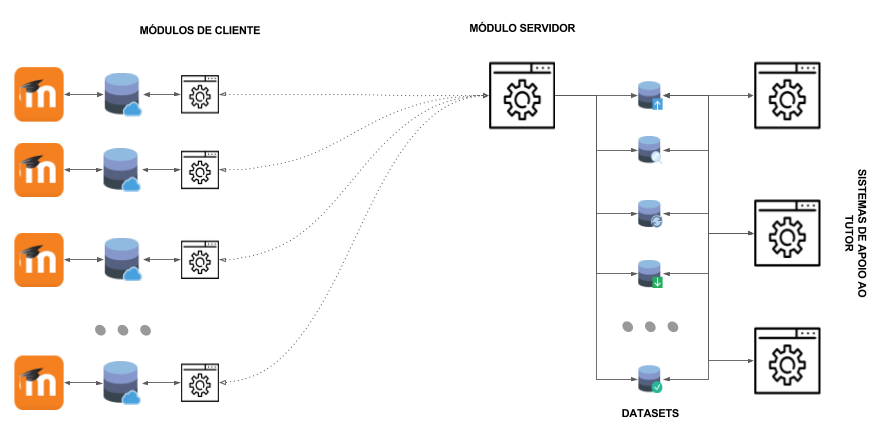
\includegraphics[width=\textwidth]{figuras/framework-moodle.png}
\caption{\textit{Framework} de transferência de dados, interligando plataformas AVA e as ferramentas de EDM.}
\label{fig-framework}
\end{figure}

A Figura \ref{fig-framework} apresenta os métodos de extração de informação dos sistema com os AVA. Inicialmente, o módulo de transferência de dados é configurado em ambas as partes, no cliente AVA e no servidor de processamento. Com a configuração, o módulo acessa cada cliente e transfere as atividades ao qual os professores marcaram para análise. O \textit{p}Nota avalia o conjunto de atividades e na primeira etapa realiza a requisição de anotação (avaliação) de amostras para treinamento do algoritmo de avaliação. O módulo de transferência envia marcações nas respostas requisitadas e o professor as avalia em seu ambiente de ensino. O sistema mantém sincronizada a versão da avaliação do professor e a versão no servidor. Em um segundo momento, com todas as respostas requisitadas já avaliadas, o sistema avaliador é treinado e recria o método de avaliação em modelos de classificação / regressão conforme as notas atribuídas. Os resultados, somando as notas atribuídas e os \textit{feedbacks} gerados, são enviados para a plataforma de ensino novamente.

O professor, em qualquer momento fica aberto para finalizar/cancelar o processamento ao liberar a chave de buscas em sua plataforma. Da mesma forma, a nota atribuída pelo professor é considerada a correta, sendo objetivo do sistema atender seu modelo avaliativo. Assim, é livre ao professor a alteração e controle de qualquer nota mesmo que ainda em processo de análise do sistema. Portanto, o professor a todo momento fica responsável por monitorar o processo avaliativo e ajustar os resultados propostos pelo sistema. A análise textual, seleção de amostras, modelos avaliativos e materiais explicativos aplicados pelo \textit{p}Nota em cada atividade são apresentadas detalhadamente em quatro etapas do processo de correção automática.

\section{Extração das Componentes Textuais}
\label{sec-componentes-textuais}

A primeira etapa, denominada de extração de componentes textuais, compreende a análise do conteúdo textual para a extração de conhecimento. Com os documentos organizados, o primeiro processo é a leitura do modelo de dados. Foram observados 3 diferentes modelos de dados: um único arquivo para todo o \textit{dataset} da atividade, um arquivo de resposta textual para cada estudante em uma coleção para a atividade e, por fim, uma estrutura por aluno que contém os arquivos enviados para a com o conteúdo textual do aluno para a atividade. Com o carregamento dos arquivos, cada aluno é representado pelo seu identificador, seja ele uma referência da plataforma de origem ou sua respectiva ordem na estrutura do \textit{dataset}.

Após a leitura do conjunto de dados, o sistema realiza uma série de processos de padronização, segmentação, filtragem, transformação e vetorização dos documentos. As etapas são sequenciais e encadeadas para análise do conteúdo em diferentes níveis. A padronização é composto pela coleta do conteúdo da resposta, remoção de conteúdos extras que permeiam o texto e a garantia da equivalência na ocorrência de cada termo. A segmentação visa a construção de vetores de resposta, termo-a-termo, identificando séries de \textit{tokens} através de uma heurística cada palavra que a compõe. A filtragem, a partir dos vetores de resposta, seleciona as palavras com potencial relação com o conteúdo. A transformação compreende extrair as estruturas das componentes textuais e modificar cada palavra para um token representante. Por fim, com os documentos padronizados, ocorre a vetorização, analisando a frequência de \textit{tokens} ou séries de \textit{tokens} para representarem o conteúdo da submissão do aluno.

\subsection{Padronização}
\label{subsec-padronizacao}
% STD_MTH = ["accents", "punct", "spaces", "tags"]
Com a extração do texto do documento enviado pelo aluno, o conteúdo, neste primeiro momento, está em estado bruto. No estado bruto o documento precisa ser normalizado seguindo um padrão para os diferentes espaçamentos, acentuação e pontuação. Além disso, é fundamental remover conteúdos não interpretáveis incluindo caracteres não alfanuméricos e \textit{tags} (marcações). Portanto, esta etapa é composta pelos seguintes processos:

\begin{itemize}
	\item Remover acentuação;
	\item Remover caracteres não-alfanuméricos;
	\item Remover pontuação;
	\item Remover espaços extras;
	\item Remover marcações.
\end{itemize}

Após cada um dos processos o conteúdo do aluno está normalizado para as próximas etapas. Os sinais gráficos auxiliam na identificação, pronúncia e leitura dos termos. Porém, computacionalmente, os sinais gráficos não é relevante para identificação de cada termo. O inverso ocorre com marcações de arquivos estruturados. As marcações, apesar da interpretação computacional, não fazem parte do conteúdo produzido pelo estudante. Portanto, ambos os casos não adicionam semanticamente ao conteúdo das respostas.

\subsection{Segmentação}
\label{subsec-segmentacao}
% TKN_MTH = ["simple", "word", "regex", "informal"]

A partir dos documentos em formato padrão, com o texto normalizado, é possível partir para análise detalhada do conteúdo. Segmentações comuns podem particionar o conteúdo por palavras, por caracteres, por frases ou por parágrafos. Cada particionamento tem um aspecto específico alinhado com as tarefas realizadas na sequência. Neste caso, a análise detalhada do conteúdo depende do particionamento do que foi obtido em segmentos de palavras. Cada segmento é denominado \textit{token}. Os \textit{tokens}, neste caso, representam as palavras separadas por uma heurística, que delimita de cada segmento. Uma heurística simples é a \textit{tokenização} por espaçamento, porém, como é um método simples é sujeito a muitas falhas. Apesar disso, métodos com melhor desempenho compreendem a aplicação da linguagem e consideram formas específicas de pontuação ou divisões do estilo textual.

A segmentação é o método que transforma o conteúdo em uma lista de palavras. A sequência de palavras permite que os próximos níveis trabalhem a perspectiva de cada \textit{token} desta lista ou sua vizinhança. É muito comum que, durante o processo, o documento seja manipulado de diferentes formas, inclusive passando várias vezes pela transformação de texto em lista de \textit{tokens} e vice-versa. Deste modo, os \textit{tokens} permitem que cada palavra seja trabalhada de forma independente, sem impactar no conteúdo adjacente.

\subsection{Filtragem}
\label{subsec-filtragem}
% FLT_MTH = ["smallwords", "stopwords", "largewords", "numerals"]
A filtragem de conteúdo é uma etapa muito importante desse processo. Uma dificuldade da filtragem é o balanceamento para alcançar níveis desejáveis de aquisição de informação. Portanto, como esperado, a filtragem estabelece uma grande perda de informação e redução do conteúdo dos documentos. Entretanto, vale ressaltar que a perda de informação inerente ao processo caracteriza uma melhoria na consistência e na equivalência dos documentos. Como é uma limpeza conduzida pelo sistema, as características removidas representam detalhes com baixa correlação com a essência de cada resposta.

Em geral, nem todos os termos de uma sentença fazem parte do núcleo de interesse para análise das respostas. Algumas palavras independem do contexto ao qual são empregadas e não são aderentes ao tema. Esse é o caso das \textit{stopwords}. As \textit{stopwords} são palavras que são empregadas na linguagem como conectivos e não representam o conteúdo passado. Assim, são extremamente importantes para a leitura e interpretação do contexto, mas não adicionam informação quando empregadas. Assim, a lista de \textit{stopwords} é um método que restringe a frase a palavras com maior potencial de relação com o contexto e o tema da resposta do estudante. Outros métodos de filtragem também incluem a remoção de palavras com poucos ou muitos caracteres e com tendência a serem muito específicos, quando não se enquadram como \textit{stopwords}. Assim, podemos incluir como parte deste processo as seguintes etapas:

\begin{itemize}
	\item Remover palavras pequenas (menores que 3 caracteres);
	\item Remover palavras grades (maiores que 15 caracteres);
	\item Remover \textit{stopwords};
	\item Remover números.
\end{itemize}

A remoção de partes do conteúdo devem cautelosamente observadas para não impactarem na capacidade de análise do conteúdo. Um bom exemplo é a extração dos números de uma resposta. Este método nem sempre é utilizado pelo sistema, dada sua influência no conteúdo. De modo prático, a aplicação deste método impacta diretamente na capacidade de análise de respostas compostas por números ou datas. 

No entanto, podemos destacar a relevância da filtragem de conteúdo através de exemplos de aplicação. Por exemplo, uma situação ao qual encontramos uma fórmula em meio ao texto e, após as padronizações, se tornam comuns os caracteres soltos em meio ao texto. Neste caso, a função que elimina os \textit{tokens} com menos de 3 caracteres remove tal conteúdo descontextualizado e direciona o sistema para atentar-se no contexto descrito pelo aluno. Por outro lado, a função que elimina com mais de 15 caracteres também tem papel fundamental. Podemos tomar como exemplo respostas que o estudante insere uma série de \textit{links} como fontes do que foi descrito na resposta. Sob a perspectiva do sistema os \textit{links} são grandes palavras únicas e não-interpretáveis. Então, a remoção de palavras com uma extensão incomum visa eliminar resquícios de conteúdo como \textit{links} que não foram retirados nos níveis inciais de tratamento por conterem caracteres alfanuméricos.

Nesta etapa, portanto, os filtros de conteúdos são métodos de redução de ruído, responsáveis por discernir quais termos podem ser extraídos de cada item de resposta. O ruído em meio ao texto pode ser um grande problema para o desempenho do classificador em relação a interpretação do conhecimento. Identificando apenas a essência de cada resposta, esperamos que o sistema tenha maior capacidade de interpretativa da relação entre respostas.

\subsection{Transformação}
\label{subsec-transformacao}
% TRF_MTH = ["NER", "MORPH", "POS", "STEMM", "LEMMA"]

Em meio aos métodos de padronização, uma importante etapa é a transformação da série de \textit{tokens}. As transformações envolvem métodos complexos de NLP, treinados para classificação de cada \textit{token} segundo sua função na linguagem. Neste nível de trabalho do texto, o texto original é particionado, sendo observado em diferentes perpectivas. Os diferentes níveis analizados nesta etapa é apresentado à seguir:

\begin{itemize}
	\item Análise gramatical: \textit{Part-of-Speech Tags} (POS-Tags);
	\item Análise semântica:\textit{Named Entity Recognition} (NER);
	\item Análise morfológica;
	\item Modificação: \textit{Stemming};
	\item Modificação: \textit{Lemmatization};
	\item Modificação: Tipografia.
\end{itemize}

Cada uma das atividades aplica uma diferente transformação no texto. Os primeiros três níveis, analíticos, acrescentam diversidade na informação de cada \textit{token} do texto. O primeiro, usando \textit{POS-Tags} realiza a análise gramatical de toda sequência. O método \textit{POS-Tag} classifica cada palavra segundo sua função no âmbito gramatical, dentre verbos, adjetivos, pronomes, dentre 17 categorias \cite{marneffe2021}. Em nível semântico, o NER é uma atividade de identificação de entidades nomeadas em meio ao texto livre \cite{pirovani2019}. Através do NER, categorias de nomes são definidas conforme a instância ao qual ele representa. Dentre as categorias reconhecidas neste trabalho estão \textit{pessoa} (PER), \textit{local} (LOC), \textit{organização} (ORG) e \textit{diversos} (MISC). Por último, o analisador morfológico identifica detalhes na construção de cada palavra. Pela análise morfológica certas palavras são identificadas segundo sua flexão. Dentre as flexões classificadas por cada termo estão as nominais (como gênero, número e definição) e verbais (pessoa, modo, tempo, voz). Adicionalmente, esse módulo também realiza algumas classificações léxicas de pronomes, adjetivos e advérbios \cite{marneffe2021}.

Com análises linguísticas complexas, cada \textit{token} é observado em diferentes perspetivas. Adicionalmente, para lidar com o texto em si, aplicamos três tipos de modificadores. Os modificadores alteram o texto original para adicionar mais uma padronização. Aqui, no entanto, a padronização torna a linguagem mais próxima da compreensão do sistema do que da linguagem humana. Inicialmente, o processo de modificação de tipografia (\textit{case}) torna todo o texto em letras maiúsculas ou minúsculas. Ao realizar essa mudança o sistema define palavras equivalentes para uma mesma forma. Do mesmo modo, os processos de \textit{stemming} e \textit{lemmatization} extraem das palavras flexionadas suas formas básicas \cite{baeza2011}. A forma simplificada extraída através do processo de \textit{stemming} é a raiz da palavra. Enquanto isso, a simplificação resultante do processo de \textit{lemmatization} é o \textit{lemma} da palavra, ou seja, sua forma sem flexões. Em ambos os casos os \textit{tokens} são modificados e todas as palavras de uma mesma base são dadas como coincidentes.

A resultante desses processos é uma forte análise das componentes textuais de cada documento de forma a compreender a construção do texto \cite{spalenza2020}. Através dessas verificações textuais, o texto recebe adição de diversos modelos que, em conjunto, caracterizam a construção termo-a-termo de cada frase. Os módulos analíticos, ampliam a informação de cada documento, tornando as nuances da escrita uma variável de interesse. Enquanto isso, os demais módulos visam aumentar a compatibilidade entre documentos para que escritas similares sejam trabalhadas de modo uniforme. Assim, o sistema como avaliador é responsável por compreender que o \textit{corpus} foi trabalhado em diferentes perspectivas. Os termos são uma referência que buscam alinhamento com a resposta esperada na avaliação. Por outro lado, a estrutura frasal representa diferentes níveis linguísticos da escrita do estudante.

\subsection{Vetorização}
\label{subsec-vetorizacao}

A vetorização, como última etapa do pré-processamento, é responsável por extrair o modelo numérico de cada documento, permitindo mensurar a diferença ou equivalência para os demais itens da coleção. Deste modo, os documentos são representados por vetores numéricos segundo seu padrão de características. Cada uma das características é analisada conforme sua frequência de ocorrência em cada documento do \textit{dataset}. A representação vetorial numérica de cada documento pela frequência é denominada \textit{Term Frequency} (TF). Sendo a coleção de documentos $ D = { d_{0}, d_{1}, d_{2}, \hdots d_{i} } $ e as características (\textit{features}) encontradas nos documentos $ F = { f_{0}, f_{1}, f_{2}, \hdots f_{j} } $.  Portanto, para cada documento $ d $ na coleção $ D $, contamos a frequência de cada \textit{feature} $ f_{j} $ do vocabulário $ F $. Deste modo, a forma vetorial do documento de índice $ i $ é dada por $ d_{i} $, sendo o vetor composto pela frequência $ n $ de cada \textit{feature} no documento $ n_{i, j} $. Então, podemos representar cada documento em $ D $ por sua forma vetorial $ d_{i} = { n_{i, 0}, n_{i, 1}, n_{i, 2} \hdots n_{i,j}} $, usando TF.

Dada as diferenças entre a frequência de cada termo em cada documento, é aplicada a pondereção para equilibrar a relação de frequência. A ponderação é denominada \textit{Inverse Document Frequency} (IDF). O \textit{Term Frequency-Inverse Document Frequency} (TF-IDF) estabelece a relação de que termos que ocorrem em muitos documentos têm menor relevância \cite{baeza2011}. A ponderação ocorre conforme a Equação \ref{eq-tfidf}.

\begin{equation}
TF-IDF = d_{i,j}* \log \frac{n_{D}}{n_{d_{j}}}
\label{eq-tfidf}
\end{equation}


Portanto, o IDF é uma ponderação na frequência de cada \textit{feature} no vetor $ d_{i, j} $, segundo o total de documentos $ n_{d_{j}} $ que contém $ f_{j} $ em relação ao total de documentos da coleção $ D $. Essa ponderação reduz a diferença numérica entre uma característica encontrada em todos os documentos para as características que estão em grupos de documentos. Assim, o uso deste modelo potencialmente delimita melhor características relevantes em avaliações com mais gradações de notas. Então, a aplicação deste modelo está diretamente associada à capacidade de identificação de características com alta correlação a grupos específicos de nota.

No método de vetorização, durante a verificação de frequência de cada característica, existe a preocupação de manter a relação de vizinhança entre os termos e sua construção sequencial. Assim, para preservar o aspecto textual em sequências e identificar características adjacentes com alta correlação, utilizamos a análise por \textit{n-grams}. Através dos \textit{n-grams}, em vez de cada documento ser representado por um vetor simples da frequência de cada característica, essa frequência é calculada segundo uma sequências de $ n $ termos. Sendo aplicado valores $ n $ de 1 a 5-\textit{grams}, utilizamos sequencias de 1 até 5 termos para analisar comportamento de cada documento em cada uma de suas perspectivas textuais. Portanto, as diferentes componentes textuais identificadas através de \textit{n-grams} em busca de padrões mais complexos e associações de termos fortemente correlatos ao método avaliativo \cite{spalenza2020}.

\section{Particionamento do Conjunto de Respostas}
\label{sec-amostragem}

A partir dos vetores de documentos, o sistema \textit{p}Nota torna-se capaz de comparar itens de resposta segundo suas componentes textuais. Com as características em formato numérico, começamos a interagir com o professor em busca da criação dos modelos que relacionem os documentos com as notas atribuídas. Entretanto, para criação destes modelos, o sistema precisa receber avaliação de alguns documentos para estabelecer a relação entre o que é o conteúdo de cada documento e a nota ao qual cada um recebe. Apesar de que muitos sistemas realizam uma amostragem aleatória, o \textit{p}Nota realiza uma amostragem baseada na distribuição dos vetores. A análise da distribuição dos vetores e suas características é dada por meio de métodos de \textit{clusterização}.

\subsection{Clusterização}
\label{subsec-clusterizacao}

A \textit{clusterização} é realizada com a otimização segundo o \textit{elbow method}. Esse método é designado por testar sequência de valores de parâmetros para identificar a melhor combinação de \textit{clusters} segundo uma métrica de qualidade. Em geral, a métrica de qualidade é diretamente relacionada com o propósito de uso dos \textit{clusters}. O algoritmo de \textit{clusterização} utilizado é o \textit{Agglomerative Clustering} \cite{spalenza2019}, um método hierárquico de agrupamento por proximidade. O \textit{Agglomerative} compreende formar \textit{clusters} agrupando item a item até que um limiar de proximidade seja alcançado dado um $ k $ número de \textit{clusters} \cite{everitt2011}.

Dentre as métricas estudadas estão o \textit{Calinski-Harabasz Score} (CHS) \cite{calinskiharabasz1974}, \textit{Davies-Bouldin Score} (DBS) \cite{daviesbouldin1979}, \textit{Silhouette Score} (SS) \cite{rousseeuw1987} e \textit{Sum of Squared Errors} (SSE) \cite{maimon2005}. Essas métricas são denominadas índices de validação interna e avaliam os agrupamentos sem considerar a anotação de cada amostra, ou seja, de modo não-supervisionado. Cada índice é uma heurística utilizada para mensurar, sob diferentes perspectivas, a qualidade dos \textit{clusters} gerados em relação a outros agrupamentos em um mesmo \textit{dataset}. CHS mensura a razão entre a dispersão dos itens intra-\textit{cluster} e a dispersão extra-\textit{cluster}. DBS é o indice que estabelece a relação entre a média de similaridade entre as amostras do \textit{cluster} para a média de similaridade entre-\textit{clusters}. O SS é a média entre as distâncias das amostras pertencentes a um \textit{cluster} em relação às amostras do \textit{cluster} mais próximo. Por fim, SSE é uma métrica que avalia o erro de cada amostra que compõe um \textit{cluster} em relação ao seu centróide. O centróide é o ponto médio dos itens que constituem cada \textit{cluster}. Portanto, o centróide é uma instância representante da dispersão dos itens no \textit{cluster}, porém é um ponto artificial e não necessáriamente uma amostra que o compõe.

Para a avaliação de respostas abertas, consideramos que o ideal são as análises que balanceam os itens de cada \textit{cluster} em relação aos \textit{cluters} adjacentes. Por padrão escolhemos a análise de \textit{silhouette}, para identificar os resultados de \textit{clusterização} com maior separabilidade entre os \textit{clusters}. A separabilidade indica se os \textit{clusters} formados são bem definidos, consistentes e sem sobreposição. Nesse índice, valores próximos a 1,0 representam agrupamentos consistentes, com distância para o \textit{cluster} mais próximo. Valores negativos, aproximando-se de -1,0, indicam aleatoriedade na associação entre \textit{clusters} e amostras, com confusão entre as os agrupamentos. Por outro lado, valores próximos a 0,0 indicam sobreposição entre \textit{clusters}, com itens no limiar de pertencer diferentes grupos. 

Em relação a verificação dos coeficientes de SS, a otimização com \textit{elbow-method} identifica no intervalo de busca qual maximiza o resultado do índice. A otimização utiliza \textit{Gaussian Process} para redução das possibilidades de busca. Esse método analisa cada teste pela distribuição dos valores da métrica de qualidade como uma \textit{gaussiana}, buscando pontos de máxima da função. A resultante é dada pelo melhor valor encontrado \cite{spalenza2019}. O atributo de controle é o $ k $, número de \textit{clusters}. O intervalo de $ k $ é definido por valores de $ 2 $ até $ 2 * \sqrt{n} $, sendo $ n $ o número de amostras do \textit{dataset} \cite{han2011}. Simultaneamente, para cada combinação de $ k $ são realizados testes com vinte métricas de distância.

\begin{itemize}
\begin{multicols}{4}
  \item braycurtis
  \item canberra
  \item chebyshev
  \item correlation
  \item cosine
  \item dice
  \item euclidean
  \item hamming
  \item haversine
  \item jaccard
  \item kulsinski
  \item mahalanobis
  \item manhattan
  \item matching
  \item minkowski
  \item rogerstanimoto
  \item russellrao
  \item sokalmichener
  \item sokalsneath
  \item yule
  \end{multicols}
\end{itemize}

A resultante da otimização em clustering é escolhida como o teste que apresenta a melhor coeficiente de SS e com maior número de \textit{clusters} formados. Enquanto o SS avalia a separabilidade dos agrupamentos, o maior número de \textit{clusters} formados indica, na perspectiva do modelo avaliativo, uma possível coincidência entre conteúdo e notas. O agrupamento selecionado é utilizado para amostragem em um percentual do conjunto de respostas disponíveis. Para avaliar qualitativamente os resultados de \textit{clusterização} utilizamos os índices \textit{Adjusted Rand Index} (ARI), \textit{Normalized Mutual Information} (NMI) e \textit{Clustering Accuracy} (CA) \cite{spalenza2019}.

O ARI é um índice que compara a similaridade entre dois \textit{clusters} de dados, levando em consideração o rótulo atribuído a cada amostra segundo seu agrupamento. Desta forma, o ARI estabelece uma relação entre pares de grupos formados e os rótulos reais de cada amostra, considerando possíveis inversões nos agrupamentos resultantes. Em geral, essa similaridade (\textit{rand-index}) poderia ser calculada sem os rótulos, mas neste caso o índice é ajustado pela expectativa de ocorrência das classes. Portanto, o ajuste é dado com a associação entre cada classe $ d_{y} $ e sua representação segundo o \textit{cluster} $ c_{i} $. A Equação \ref{eq-ARI} apresenta o cálculo realizado por cada um deste índices de \textit{clusterização}.

\begin{equation}
ARI = \frac{RI - Expected_{(RI)}}{MAX_{(RI)} - Expected_{(RI)}}
\label{eq-ARI}
\end{equation}

\begin{equation*}
RI = \frac{\sum_{i=1}^{C} d_{y} == c_{i}}{D}
\end{equation*}

De modo distrinto, NMI estabelece uma escala de correlação entre os rótulos das amostra e a associação de cada uma a um cluster. Nesse aspecto, NMI relaciona a categoria aos \textit{clusters} formados segundo sua coesão, segundo a Mutual Information (MI) e a Entropia (H) obtidas entre \textit{clusters} (c) e classes (y). Em destaque, H é dado pelo somatório das probabilidade de cada classe $ y $ no conjunto, enquanto MI é dada pela diferença entre a entropia global $ H_{(y)} $ e a entropia do grupo em análise $ H_{(y, c)} $. Essa relação de NMI para MI e H é dada pela Equação \ref{eq-NMI}.

\begin{equation}
NMI_{(y,c)} = \frac{2*MI_{(y,c)}}{H_{(y)}+H_{(c)}}
\label{eq-NMI}
\end{equation}

Sendo:

\begin{equation*}
MI_{(y, c)} = H(y) - H_{(y, c)} 
\end{equation*}

\begin{equation*}
H_{(y)} = \sum_{i=1}^nP(y_{i})\log_{2}(P(y_{i}))
\end{equation*}

E, por fim, utilizamos a CA para avaliar a categorização por voto majoritário dos grupos formados. Assim, com CA verificamos se os \textit{clusters} são formados majoritáriamente por uma classe e, verificar a separação entre as classes. A Equação \ref{eq-CA} apresenta a contagem das amostras d com determinada classe y para cada um dos C \textit{clusters} formados.

\begin{equation}
CA = \frac{\sum_{i=1}^{C} MAX(d_{(y, c_{i})})}{D}
\label{eq-CA}
\end{equation}

Com os índices de qualidade de \textit{clusterização}, estabelecemos uma perspectiva dos resultados esperados com os grupos formados e as categorias atribuídas pelo professor. Em especial, os índices foram utilizados como parâmetro para mensurar o impacto de \textit{clusterizações} homogêneas e aprimorar a amostragem para posterior classificação. Deste modo, podemos estudar formas de seleção mais robusta de amostras após a formação de \textit{clusters}.


\subsection{Seleção de Amostras}
\label{subsec-selecao-amostras}

Com a formação dos \textit{clusters}, buscamos identificar as principais respostas de cada agrupamento para coleta do modelo avaliativo do professor. A amostragem é realizada com a coleta de um percentual dos itens que compõe o \textit{dataset}. Essa coleta analisa padrões de documentos de cada grupo, a fim de compreender como é dada a avaliação do especialista para cada um dos diferentes itens. As amostras são selecionadas conforme critérios específicos, descrevendo um padrão específico do \textit{cluster}. Os sete critérios de seleção de amostras utilizados estão listados abaixo:

\begin{itemize}
	\item Par de amostras de menor similaridade no \textit{cluster};
	\item Par de amostras de maior similaridade no \textit{cluster};
	\item Amostra com mais características do \textit{cluster};
	\item Amostra com menos características do \textit{cluster};
	\item Amostra com menor índice de \textit{silhouette} do \textit{dataset};
	\item Amostra aleatória do maior \textit{cluster};
	\item Amostra aleatória do \textit{dataset}.
\end{itemize}

As sete instâncias, seguem uma ordem de prioridade conforme o percentual de itens coletados. O par de maior e o par de menor similaridade compreendem os itens mais convergentes e mais divergentes que compõe cada \textit{cluster}. Em uma diferente perspectiva, a coleta de amostras dos itens de maior e menor número de características indicam as respostas que foram mais extensas e mais concisas, respectivamente. A coleta destes itens indica a consistência do padrão reconhecido na atribuição dos \textit{clusters}. Em \textit{clusters} com apenas um par de itens, por exemplo, todos os quatro modelos de amostragem são dados para as duas únicas amostras. Portanto, após essa seleção, não necessariamente foram identificadas 6 instâncias por \textit{cluster}. A composição de até o percentual de amostragem por \textit{dataset} é dado de três formas, aplicada conforme a demanda do sistema. A forma padrão, e mais robusta, é dada através da análise de dispersão de cada item.

A análise de dispersão calcula o coeficiente de \textit{silhouette} da amostra. Tal qual o SS, esse índice determina a razão entre a distância da amostra para os demais itens do grupo em relação aos itens do \textit{cluster} mais próximo. Desta forma, esse método incrementa as amostras por dispersão até alcançar o percentual de amostragem selecionado. Uma outra opção de seleção é a escolha de amostras por balanceamento do tamanho dos \textit{clusters}. Tal método determina que um item seja aleatoriamente selecionado, sendo a seleção ponderada de acordo com a quantidade de itens que compõe cada grupo. Por fim, caso seja descartada a análise para amostragem dos demais itens, a seleção é realizada aleatoriamente, coletando itens sem uso dos agrupamentos.

Terminando este procedimento de seleção de amostras, as representantes de cada grupo são enviadas para avaliação do professor no papel de especialista. O especialista é responsável por atribuir notas de acordo com seu método avaliativo. Fica a cargo do próprio sistema identificar como os padrões de nota estão alinhados com os padrões textuais das respostas. Para isso, as notas coletadas devem ser estudadas pelo sistema para identificar o alinhamento do modelo avaliativo com o conteúdo das respostas.

\section{Modelo Avaliativo}
\label{sec-avaliacao}

O desenvolvimento do modelo SAG acontece depois que o professor analisa todos as requisições de anotação, avaliando-as. Para a criação de um modelo SAG, é fundamental o desenvolvimento de um padrão de associação entre termos e notas. Entretanto, identificar os detalhes observados pelo professor na avaliação não é trivial. Através do conjunto de respostas, o \textit{p}Nota compara respostas que receberam a mesma avaliação para identificar padrões correspondentes. Os padrões encontrados em uma mesma nota, indicam detalhes que provavelmente foram levados em conta pelo professor na hora da avaliação. Deste modo, o sistema visa recuperar a expectativa de resposta por nota diante do alinhamento entre as componentes textuais.

\subsection{Classificação}
\label{subsec-classificacao}

O processo de classificação enquadra-se com notas ordinais e discretas. Em tais situações, os classificadores atuam relacionando os padrões de cada categoria de nota ao conteúdo textual das respostas não anotados pelo professor. Deste modo, de cada técnica age mensurando a similaridade entre os modelos conhecidos para os demais que o \textit{dataset} contém. Para isso utilizamos cinco algoritmos: \textit{K-Nearest Neighboors}, \textit{Decision Tree}, \textit{Support Vector Machine}, \textit{Gradient Boosting}, \textit{Random Forest} e \textit{WiSARD}.

O \textit{K-Nearest Neighboors} (KNN) é o algoritmo de classificação pela análise da vizinhança amostral. Através do KNN cada amostra é categorizada pela distribuição local dos seus $ k $ vizinhos. A atribuição do rótulo é por voto majoritário, atribuindo o mesmo valor a amostra não anotada. Diferentemente deste, o algoritmo \textit{Decision Tree} (DTR) estabelece a equivalência entre amostras, sob uma perspectiva das características que as compõe. O DTR define grupos anotados com a mesma classe pelos limiar das características que a compõe, gerando regras de decisão. As regras, elaboradas automaticamente, delimitam as principais \textit{features} segundo os valores de tendência de classe. Portanto, o processo de classificação acontece com a comparação de cada um dos itens dentre a cadeia de decisões na estrutura de árvore.

Outro tradicional algoritmo, \textit{Support Vector Machine} (SVM), estabelece uma forma distinta de observar os dados. Os dados, em grupos por categoria, formam um \textit{kernel}. O \textit{kernel}, diferente do DTR, cria modelo espacial que delimita a diferença entre categorias. Então, cada amostra, é identificada segundo sua posição em relação ao limiar de características dado o modelo representante da classe. De forma similar é aplicado o algoritmo \textit{Wilkes, Stonham and Aleksander Recognition Device} (WSD) \cite{aleksander1984, wisard2020}, conhecido como \textit{WiSARD} \footnote{wisardpkg - https://github.com/IAZero/wisardpkg}. O algoritmo produz um modelo binário de características através do registro de padrões de características. Cada padrão é reconhecido em análise sequencial de um intervalo de bits pré-definido. O modelo binário criado é comparado com as respostas não avaliadas, categorizando-as pela similaridade entre padrões. Especificamente para este algoritmo, a conversão dos vetores TF-IDF em seu formato binários foi dada com 1 \textit{bit} por característica, de acordo com a esparsidade observada em dados textuais \cite{manning1999}. Assim, dado como pré-requisito de sua aplicação, o padrão submetido é dado pela existência (valor 1) ou não (valor 0) de cada característica na resposta.

Adicionalmente, dois modelos de \textit{ensemble} foram aplicados. Os \textit{ensembles} são técnicas que combinam vários classificadores mais simples para determinar áreas de decisão mais robustas. Os classificadores simples são denominados \textit{weak learners}, em busca de detalhes na avaliação entre termos e classes. Nesse aspecto, \textit{Random Forest} (RDF), é um algoritmo que combina o método tradicional \textit{Decision Tree} com \textit{subsets} de amostras. Deste modo, o RDF combina análises parciais do conjunto de dados para definir regras de decisão mais complexas sobre a distribuição de amostras. De forma similar, o \textit{Gradient Boosting} (GBC) combina uma série de \textit{Regression Trees} para otimização diferencial da função de perda (\textit{loss}). Nessa linha, o GBC observa o gradiente da função de perda com \textit{Logistic Regression}. Nesse aspecto, com uma série de amostragens, a técnica procura minorar o erro de classificação obtido com a calibração do modelo segundo uma sequência de \textit{subsets}. 

A combinação com modelos tradicionais e técnicas de \textit{ensemble} visa potencializar a capacidade analítica do método. Com diferentes formatos de dados, a proposta deste trabalho testa diferentes modelos procurando o que melhor se adequa ao padrão avaliativo do professor. Nesse aspecto, o método de classificação é escolhido de acordo com a similaridade entre o modelo automático com o critério do professor \cite{pado2021}. Para avaliar este aspecto utilizamos o coeficiente \textit{kappa} quadrático \cite{cohen1960}. As amostras são separadas em dois grupos acordo com o \textit{Stratified K-Fold}, para mensurar a capacidade de cada algoritmo na categorização das amostras. As amostras são separadas conhecendo a distribuição entre as categorias e, a cada ciclo, cada avaliador é comparado segundo a paridade de seus resultados com o avaliador humano \cite{artstein2008}.

Na sequência, a qualidade de cada um é avaliada com 4 métricas. A \textit{Accuracy} (ACC), ou acurácia, mensura a equivalência percentual entre as avaliações. A \textit{Precision} (PRE), ou precisão, estabelece a razão entre a atribuição correta de rótulos e a quantidade de atribuições incoerentes da mesma categoria. De forma similar, a \textit{Recall} (REC), ou revocação, estabelece a razão entre a atribuição correta de rótulos e os itens de determinada categoria que foram classificados de forma incorreta. Por fim, F1 é o balanceamento entre PRE e REC, observando simultanemente os erros de e para cada classe. Este último é o único que além da avaliação média da atribuição de cada nota (macro) também é observada conforme a representatividade de cada categoria ao número total de amostras (ponderado). A Equação \ref{eq-classification} apresenta a fórmula de cada uma das métricas citadas para avaliação qualitativa dos algoritmos de classificação testados.

\begin{equation}
Accuracy = \frac{TP+TN}{TP+TN+FP+FN}
\label{eq-classification}
\end{equation}

\begin{equation*}
Precision = \frac{TP}{TP+FP}
\end{equation*}

\begin{equation*}
Recall = \frac{TP}{TP+FN}
\end{equation*}

\begin{equation*}
F{1} = \frac{2*Precision*Recall}{Precision+Recall}
\end{equation*}

Na Equação \ref{eq-classification}, vemos as fórmulas para mensurar a qualidade dos classificadores. Nelas $ T $ refere-se aos casos verdadeiros e $ F $ aos falsos. Da mesma forma, $ P $ refere-se aos casos positivos e $ N $ aos negativos. Com isso, todos os classificadores são avaliados segundo sua qualidade para divulgação dos resultados de modo a apreciar o resultado obtido. Porém, como descrito no processo de seleção, apenas o resultado que apresenta maior adequação ao modelo do professor é dado como resultado. Comparando estatisticamente os modelos, a expectativa é enviar apenas os resultados que sejam mais adequados, reduzindo as falhas no critério avaliativo do sistema.

\subsection{Regressão}
\label{subsec-regressao}

Em notas atribuídas em intervalos contínuos, são aplicados métodos de regressão. A regressão estima valores segundo o intervalo conhecido através das amostras. Os métodos buscam compreender o ajuste dos dados segundo a distribuição, elaborando o modelo minimizando o erro preditivo. Os cinco métodos de regressão aplicados são a \textit{Regressão Linear}, \textit{Lasso}, \textit{K-Nearest Neighboors}, \textit{Decision Tree} e \textit{WiSARD}.

A Regressão Linear (LNREG) é um algoritmo que avalia a tendência linear das amostras segundo sua distribuição. Essa tendência linear busca, no espaço n-dimensional das características, definir os coeficientes de reta que minimizam o resíduo entre as amostras. É importante para o algoritmo determinar uma função de tendência dos dados. Minimizar o erro através dos coeficientes da função reflete na simplificação do conjunto de dados. Entretanto, é determinante que o modelo não apresente \textit{overfitting} e um baixo desempenho com o viés dos dados de treinamento. Por outro lado, como espera-se do algoritmo, a aquisição de informação deve extrair um modelo que minimamente descreva os dados conhecidos, evitando a ocorrência de \textit{underfitting}. Assim, o modelo simplificado deve ser direcionado ao desempenho linear e não apenas à associação forte com o conjunto de treinamento. Também é utilizada uma variante do LNREG tradicional, denominada \textit{Least Absolute Shrinkage and Selection Operator - Lasso} (LSREG), que utiliza a normalização dos dados com a função $ L1 $, reduzindo a complexidade do modelo de dados e previnindo o \textit{overfitting}.

Os demais três modelos, são similares aos modelos utilizados na classificação. O \textit{K-Nearest Neighboors} (KNREG), assim como o algoritmo de classificação, observa a distribuição dos dados e define o valor resultante de acordo com a vizinhança. Assim, o resultado de cada amostra de valor desconhecido é a interpolação entre os valores das $ K $ amostras mais próximas conhecidas. De forma semelhante, \textit{Decision Tree} (DTREG) observa características semelhantes entre amostras e, por equivalência, divide em subgrupos. A subdivisão dos itens na árvore e o particionamento em subgrupos delimita regiões específicas com resultantes correspondentes por aproximação. Desta forma, após o particionamento das regiões amostrais em zonas de decisão, o valor dado para todas as amostras ali categorizadas é a média conhecida do subgrupo de treinamento. De forma similar funciona a WiSARD (WSREG), organizando registradores com as notas das respostas similares atribuindo o valor médio do registrador para respostas de padrão equivalente.

Segundo o modelo de notas contínuo, o método de avaliação dos métodos de regressão são dados através do erro da predição em relação a nota esperada. Assim, para mensurar a diferença entre a expectativa do professor e a nota resultante do sistema utilizamos o \textit{Mean Absolute Error} (MAE), o \textit{Mean Squared Error} (MSE) e o \textit{Root Mean Squared Error} (RMSE). O MAE, erro médio absoluto, mensura a resíduo absoluto entre a nota predita e a nota dada pelo professor. Em outras palavras, o MAE avalia as diferênças em módulo entre os valores obtidos, segundo o alinhamento de cada predição com a expectativa do professor. Enquanto isso, MSE ou erro médio quadrático, é uma medida do resíduo entre os valores com penalização dos erros absolutos. Assim, através do MSE erros maiores têm maior impacto no sistema quando comparados com erros de menor grau. Por fim, o RMSE ou raiz do erro médio quadrático, é a raiz quadrada do valor obtido no MSE, normalizando o erro obtido nesta métrica em relação à avaliação do professor. A Equação \ref{eq-regressao} apresenta a fórmula de cada uma das métricas utilizadas para avaliação dos métodos de regressão citados.

\begin{equation}
MAE = \sum_{i=0}^{D}|y_i-p|
\label{eq-regressao}
\end{equation}

\begin{equation*}
MSE = \sum_{i=0}^{D}(y_i-p)^2
\end{equation*}

\begin{equation*}
RMSE = \sqrt{\sum_{i=0}^{D}(y_i-p)^2}
\end{equation*}

Na Equação \ref{eq-regressao} apresentamos as fórmulas de avaliar o erro do modelo criado conforme a expectativa de nota. Assim, em cada fórmula dos itens para cada amostra $ i $ na coleção comparamos as notas atribuídas pelo avaliador humano $ y $ e pelo sistema $ p $. Apesar de serem comuns os erros entre modelos computacionais e a expectativa do especialista, é crucial para um bom avaliador automático a proximidade entre os modelos. Assim, é esperado ao sistema que o erro seja minimizado e, como descrito, seja capaz de lidar com diferentes situações. Portanto, a capacidade avaliativa do sistema e seu nível de interpretação da linguagem podem ser mais relevantes a longo prazo do que o erro apresentado em situações incomuns (outliers). Destacamos ainda que, devido o nível de subjetividade inato ao processo avaliativo, os erros são comuns em qualquer correção, inclusive entre dois especialistas humanos. Nos sistemas SAG, foram observados durante a correção entre professores até 0,66 pontos de divergência em notas de 0 a 5 ponto \cite{mohler2011}. Em uma escala de 0 a 10 pontos, representaria 1,32 pontos de divergência entre avaliadores humanos.

Para seleção do regressor mais adequado utilizamos a correlação de \textit{Pearson}. Independente do nível de erro o método selecionado deve cumprir gradações similares ao método de atribuição de notas do professor. Considerando todos os algoritmos aplicados como capazes de realizar uma avaliação, mesmo que de forma básica, o uso da correlação nos permite verificar se a gradação é equivalente ao que foi atribuído pelo professor no treinamento. Para mensurar isso antes da avaliação, particionamos as amostras anotadas com KFold. O algoritmo é treinado com dois terços das amostras coletadas e validado em um terço. Após a predição no \textit{subset} de avaliação, o modelo com maior índice de correlação observado é dado como padrão. Os resultados são gerados para todos os regressores, mas é encaminhado ao professor como resultado o de melhor correlação conhecida.

\section{Relatórios}
\label{sec-relatorios}

Após a classificação, com a atribuição de notas de todos os alunos, os relatórios são ferramentas importantes para aplicação direta em sala de aula. Os relatórios visam descrever para professores, estudantes e até desenvolvedores como é efetuada a análise das respostas, os métodos de reconhecimento de padrões e a coerência entre avaliação e modelos de resposta. Sabendo que cada modelo de resposta é até o momento uma associação entre termos e notas identificada pelo sistema, é determinante no processo de relatórios a apresentação deste modelo como descritor do método avaliativo.

Para ilustrar a produção de \textit{feedbacks} utilizamos a atividade \textit{Sandstone} da \textit{Open University} \cite{jordan2012}. Esta atividade inglesa foi extraída do curso de Introdução à Ciências \footnote{Sandstone - Open University. Disponível em https://www.open.edu/openlearn/science-maths-technology/science/geology/sandstone}. A Figura \ref{fig-sandstone-enunciado} apresenta o enunciado da questão apresentada aos alunos.

\begin{figure}[!t]
 \centering
 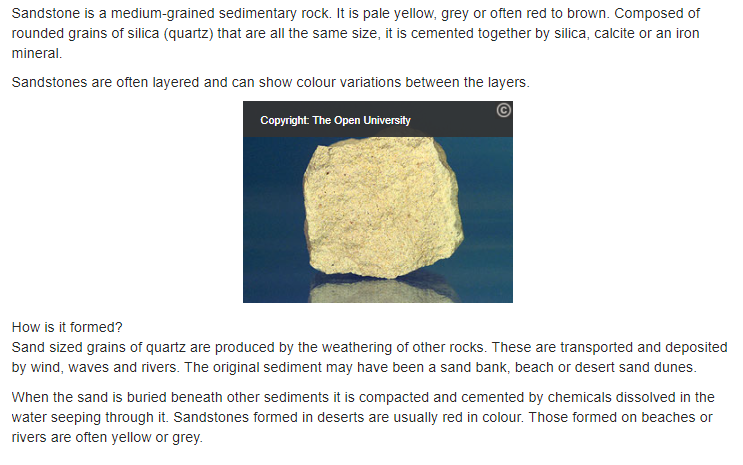
\includegraphics[width=\textwidth]{figuras/exemplo/sandstone-enunciado.png}
 \caption{Enunciado da questão \textit{Sandstone} aplicada na \textit{Open University}.}
 \label{fig-sandstone-enunciado}
\end{figure}

A atividade apresentada na Figura \ref{fig-sandstone-enunciado} faz parte da coleção disponível na \ref{cap-experimentos}. Nela os alunos devem determinar como é formado o \textit{arenito}, rocha sedmentar resultante da compactação gradual da areia. Neste conjunto o professor avaliou manualmente cada uma das 1798 respostas de forma binária, sendo 1 atribuído para resposta \textit{correta} e 0 para a \textit{incorreta}. Esta atividade é utilizada neste capítulo como exemplo para caracterizar o material recebido pelo professor como resultado. O conteúdo completo gerado para esta atividade estão disponíveis no Capítulo \ref{anexo-exemplo}. Portanto, através dos relatórios formados, discutimos os resultados obtidos nesta questão.


\begin{table}[!b]
\centering
\begin{tabular}{| c c c c |} \hline
\multicolumn{3}{|l}{Dataset} & Amostras\\ 

\multicolumn{3}{|l}{sandstone : answers.csv} & 1897\\ \hline 

 Treino (Un.) & Treino (\%)  & Teste (Un.) & Teste (\%) \\ \hline 

569 & 29.99 & 1328 & 70.01 \\ 

\hline \hline

\end{tabular}
\caption{Particionamento em amostras para treino e teste dos classificadores na atividade exemplo \textit{Sandstone}.}
\label{exemplo-train}
\end{table}

Os relatórios iniciais apresentam conteúdos e dados extraídos pelo sistema. Dentre eles estão a lista de respostas dos alunos, lista de amostras requisitadas pelo sistema, lista da frequência das principais características, descrição do particionamento de treino e teste e a descrição das \textit{features} extraídas dos documentos. Em geral, esse \textit{feedback} é um conteúdo explicativo, apresentando o que o sistema interpretou em cada documento e algumas ações básicas tomadas durante os processos como a vetorização e contagem da frequência das características. As Tabelas \ref{exemplo-train} e \ref{exemplo-feat} apresentam descrições do processamento das atividades sobre a extração de informações e particionamento de dados.

\begin{table}[!b]
\centering
\begin{tabular}{| c c c c c c c |} \hline
\multicolumn{6}{|l}{Dataset} & Amostras \\ 

\multicolumn{6}{|l}{sandstone : answers.csv} & 1897 \\ \hline 

& \multicolumn{3}{c}{Palavras} & \multicolumn{3}{c|}{Caracteres} \\ 

Caracter{\'i}sticas & Max. & Min. & M{\'e}dia & Max. & Min. & M{\'e}dia \\ \cline{2-4} \cline{5-7} 

954 & 20 & 1 & 12.7 & 166 & 3 & 77.92 \\ 

\hline \hline
\end{tabular}
\caption{Características das respostas encontradas na atividade exemplo \textit{Sandstone}.}
\label{exemplo-feat}
\end{table}


Na Tabela \ref{exemplo-train} descrevemos a forma de divisão das respostas para anotação do professor e avaliação do sistema. Por outro lado, na Tabela \ref{exemplo-feat} encontramos características sobre a extração de informação da atividade. Nela descrevemos o total de características encontrados e os padrões de resposta, tamanho máximo, mínimo e médio segundo quantidade de palavras e caracteres. Associada as listas de respostas, \textit{clusters} e amostras procuramos representar o conteúdo identificado pelo sistema e, consequentemente, explicar a etapa inicial do processamento com o \textit{p}Nota.

Outro relatório inclui a descrição do modelo avaliativo de acordo com cada um dos algoritmos testados. Independente do formato aplicado, o uso das métricas, matrizes de confusão e a comparação do desempenho de cada algoritmo ilustra a entrega de resultados do sistema. Assim, conforme os resultados finais apresentados ao fim do processo avaliativo, podemos acompanhar também a capacidade do modelo de avaliação automática gerado pelo sistema. Em diferentes perspectivas, podemos vislumbrar a capacidade de cada algoritmo avaliador. Entretanto, como principal interessado no ajuste avaliativo, destacamos a relevância do \textit{p}Nota ilustrar a efetividade do processo avaliativo diretamente ao professor. Assim, para além de mensurar a qualidade como classificador, alinhamos os objetivos do sistema com a expectativa de resultados do professor \cite{nascimento2020}. Para auxiliar a interpretação, dividimos em três categorias a avaliação automática sob a ótica do professor:

\begin{itemize}
	\item Intervalo de 75 - 100\%: Nível Avançado;
	\item Intervalo de 36 - 75\%: Nível Adequado;
	\item Intervalo de 0 - 35\%: Nível Insuficiente.
\end{itemize}

Em nível \textit{Insuficiente} a relação entre as notas finais divulgadas pelo professor e a predição do teste para o conjunto tem desempenho baixo. Em nível \textit{Adequado} as notas apresentam aprendizado das notas e modelos avaliativos alinhados com o professor. Por fim, em nível \textit{Avançado}, o desempenho do classificador automático para as demais notas foi similar ao humano, identificando bem o método avaliativo do professor. É importante também descrevermos o detalhe que cada uma das métricas utilizadas pelo sistema sob a ótica do professor \cite{nascimento2020}:

\begin{itemize}
	\item ACC: apresenta ao professor a quantidade percentual de respostas que foi avaliada de forma equivalente em relação a sua expectativa avaliativa. Através da acurácia identificamos o percentual de verdadeiros positivos, ou seja, alunos que receberam notas iguais para ambos os avaliadores, em relação ao total de respostas avaliadas. Em uma outra perspectiva podemos também considerar que, com o uso do sistema, é o percentual de notas não alteradas pelo professor após a avaliação automática.

	\item PRE: apresenta ao professor o percentual de acertos do total de amostras da avaliação automática em relação a sua expectativa avaliativa. A precisão exibe a quantidade de notas avaliadas de forma equivalente (verdadeiros positivos) em relação ao índice de notas que incorretamente avaliadas com o mesmo nível de nota (falsos positivos). Em geral, essa métrica determina ao professor o desempenho médio do sistema na avaliação de cada uma das notas atribuídas.

	\item REC: apresenta ao professor, em percentual, a capacidade do sistema em discernir cada um dos níveis de nota. A revocação é um indicativo da quantidade de notas avaliadas corretamente (verdadeiros positivos) em relação aos itens que foram categorizados de forma incoerente em outras categorias (falsos negativos). Portanto, é uma métrica que determina ao professor a capacidade média do modelo avaliativo segundo os modelos de cada nota.


	\item F1: é uma ponderação entre as métricas PRE e REC. Indica ao professor, em âmbito geral, a capacidade dos modelos avaliativos na identificação dos padrões de nota. Deste modo, é uma métrica que leva em conta os erros (falsos positivos e falsos negativos) do sistema entre as categorias em relação a coerência do modelo adquirido para os níveis de nota (verdadeiros positivos e verdadeiros negativos).

	\item MAE: apresenta ao professor o nível de erro do sistema. O erro médio absoluto determina para o conjunto de notas qual foi a diferença entre as notas atribuídas pelo professor e pelo avaliador automático. A resultante é a variação média entre as notas do professor e do sistema.

	\item MSE: apresenta ao professor o nível de erro do sistema com penalização. O erro médio quadrático determina a diferença entre as notas do professor e do sistema. Entretanto, a diferença quadrática entre notas atribui maior peso aos modelos avaliativos que apresentam discrepâncias maiores entre notas. A resultante, portanto, é a variação média entre notas do professor e do sistema após a penalização.

\end{itemize}

Em um contexto geral, os níveis e as métricas representam uma associação entre a consistência de cada avaliação dada pelo sistema automático e a representatividade do modelo de notas. Assim, podemos interpretar os erros sob duas perspectivas determinantes para a melhoria avaliativa e o bom uso do sistema. A primeira é a concordância entre a correção e as componentes textuais das respostas analisadas pelo \textit{p}Nota. E a segunda é a capacidade de montar modelos com a quantidade de respostas por cada nível de nota. O modelo formado, portanto, precisa de conteúdos coincidentes em relação aos padrões linguísticos e os modelos de nota para demonstrar o aprendizado e realizar uma avaliação efetiva. Assim, os níveis de aprendizado, \textit{Avançado}, \textit{Adequado} e \textit{Insuficiente}, descrevem como cada um dos algoritmos de classificação ou regresssão foi capaz de compreender o vínculo entre as componentes textuais e o método avaliativo. Ilustramos na Figura \ref{fig-sandstone-clf}, através da atividade selecionada como exemplo, os três níveis de aprendizado.

\begin{figure}[!h]
\begin{minipage}[t]{.5\textwidth}
 \centering
 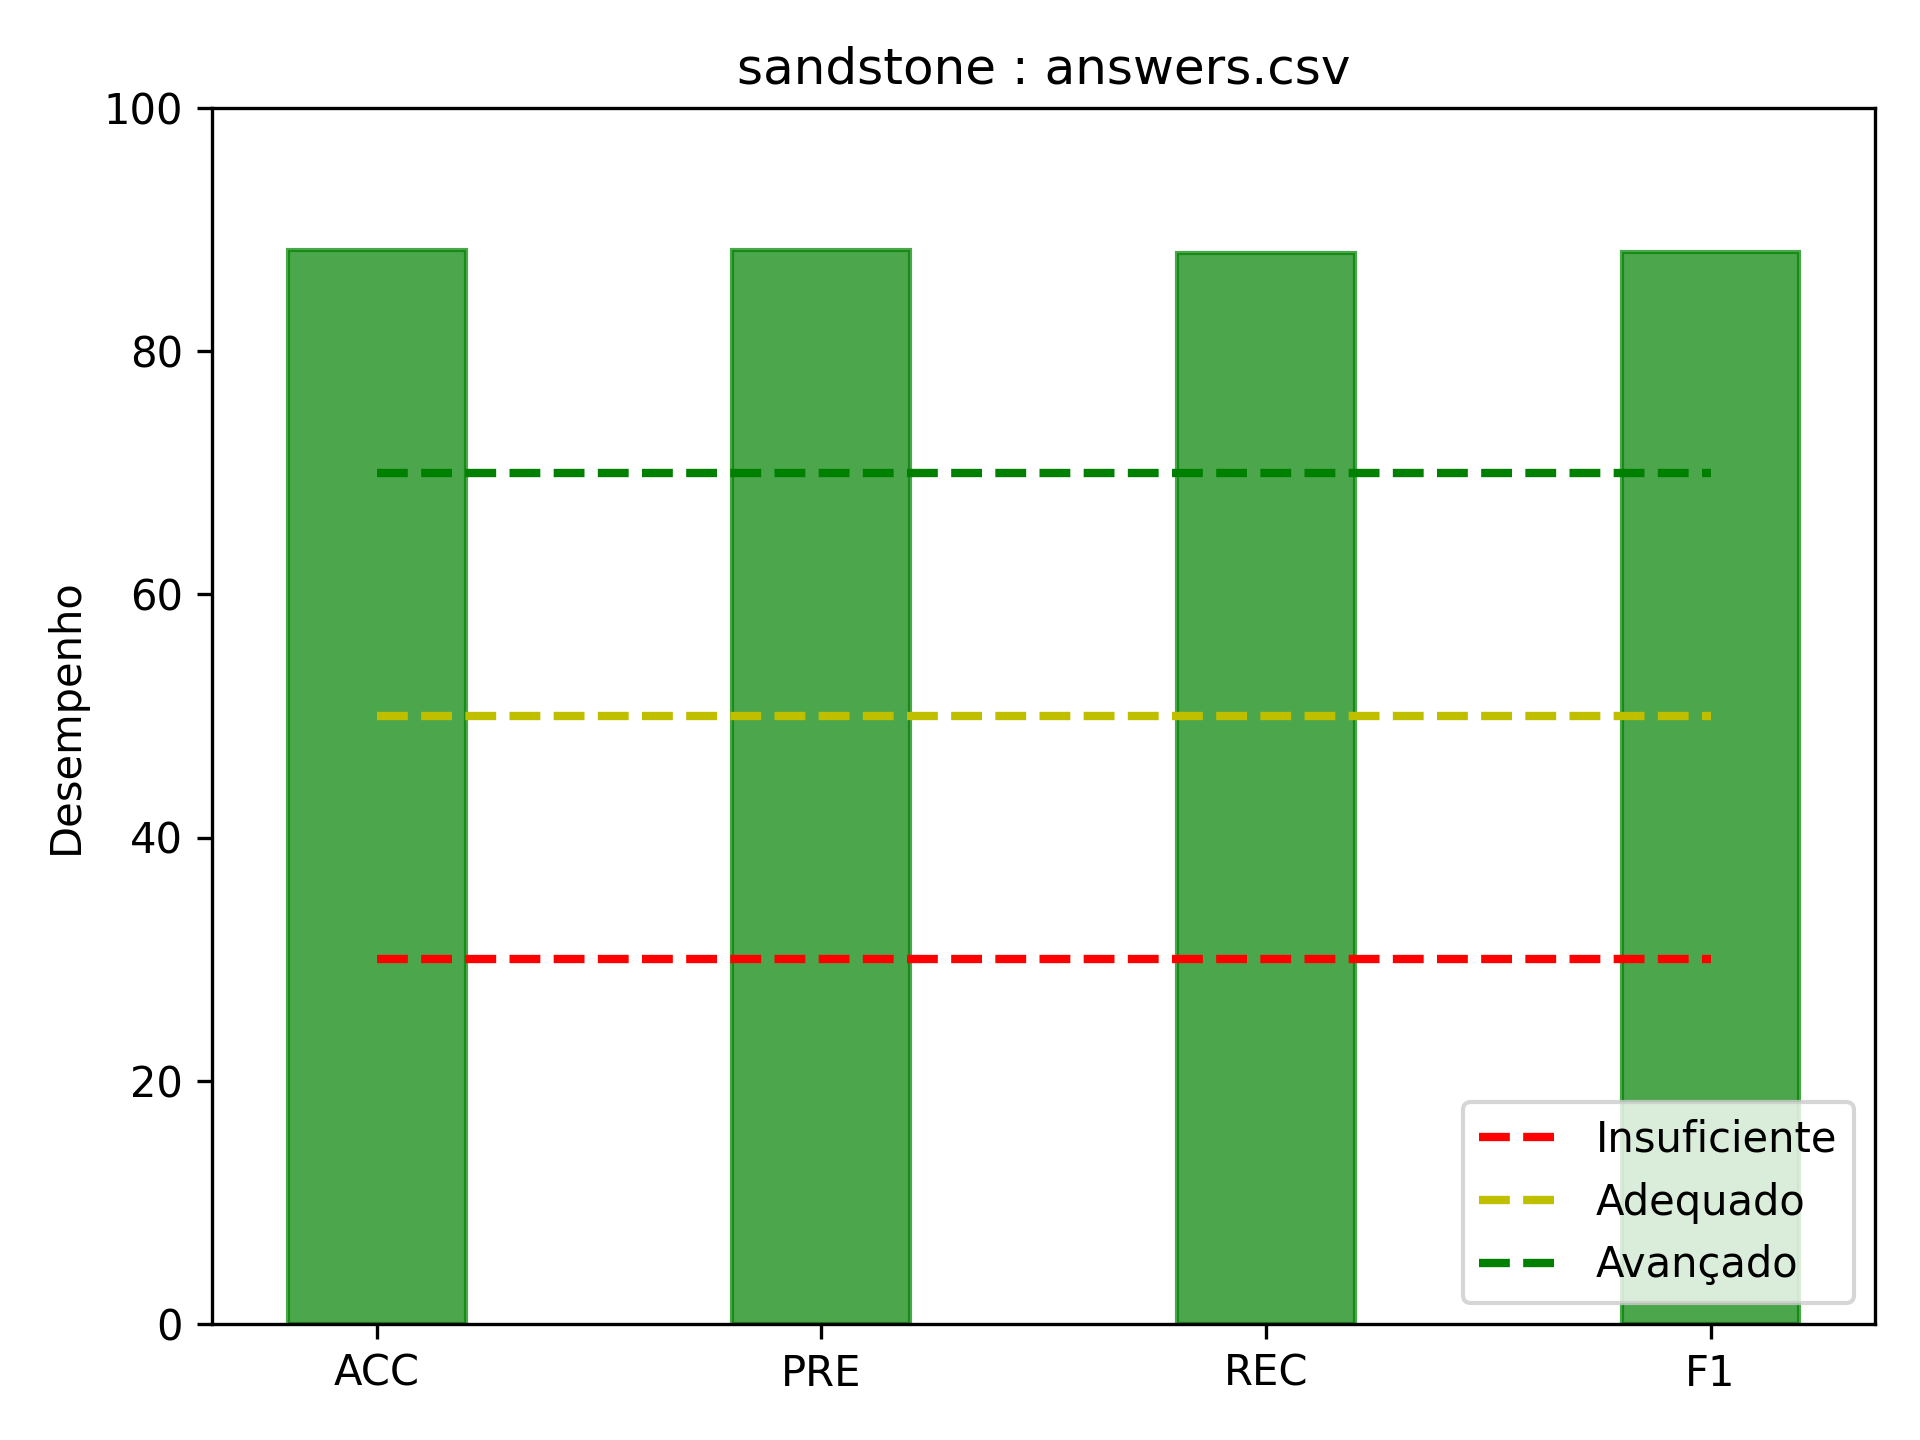
\includegraphics[width=\textwidth]{figuras/exemplo/sandstone-evalRDF.png}
\end{minipage}
\begin{minipage}[t]{.5\textwidth}
 \centering
 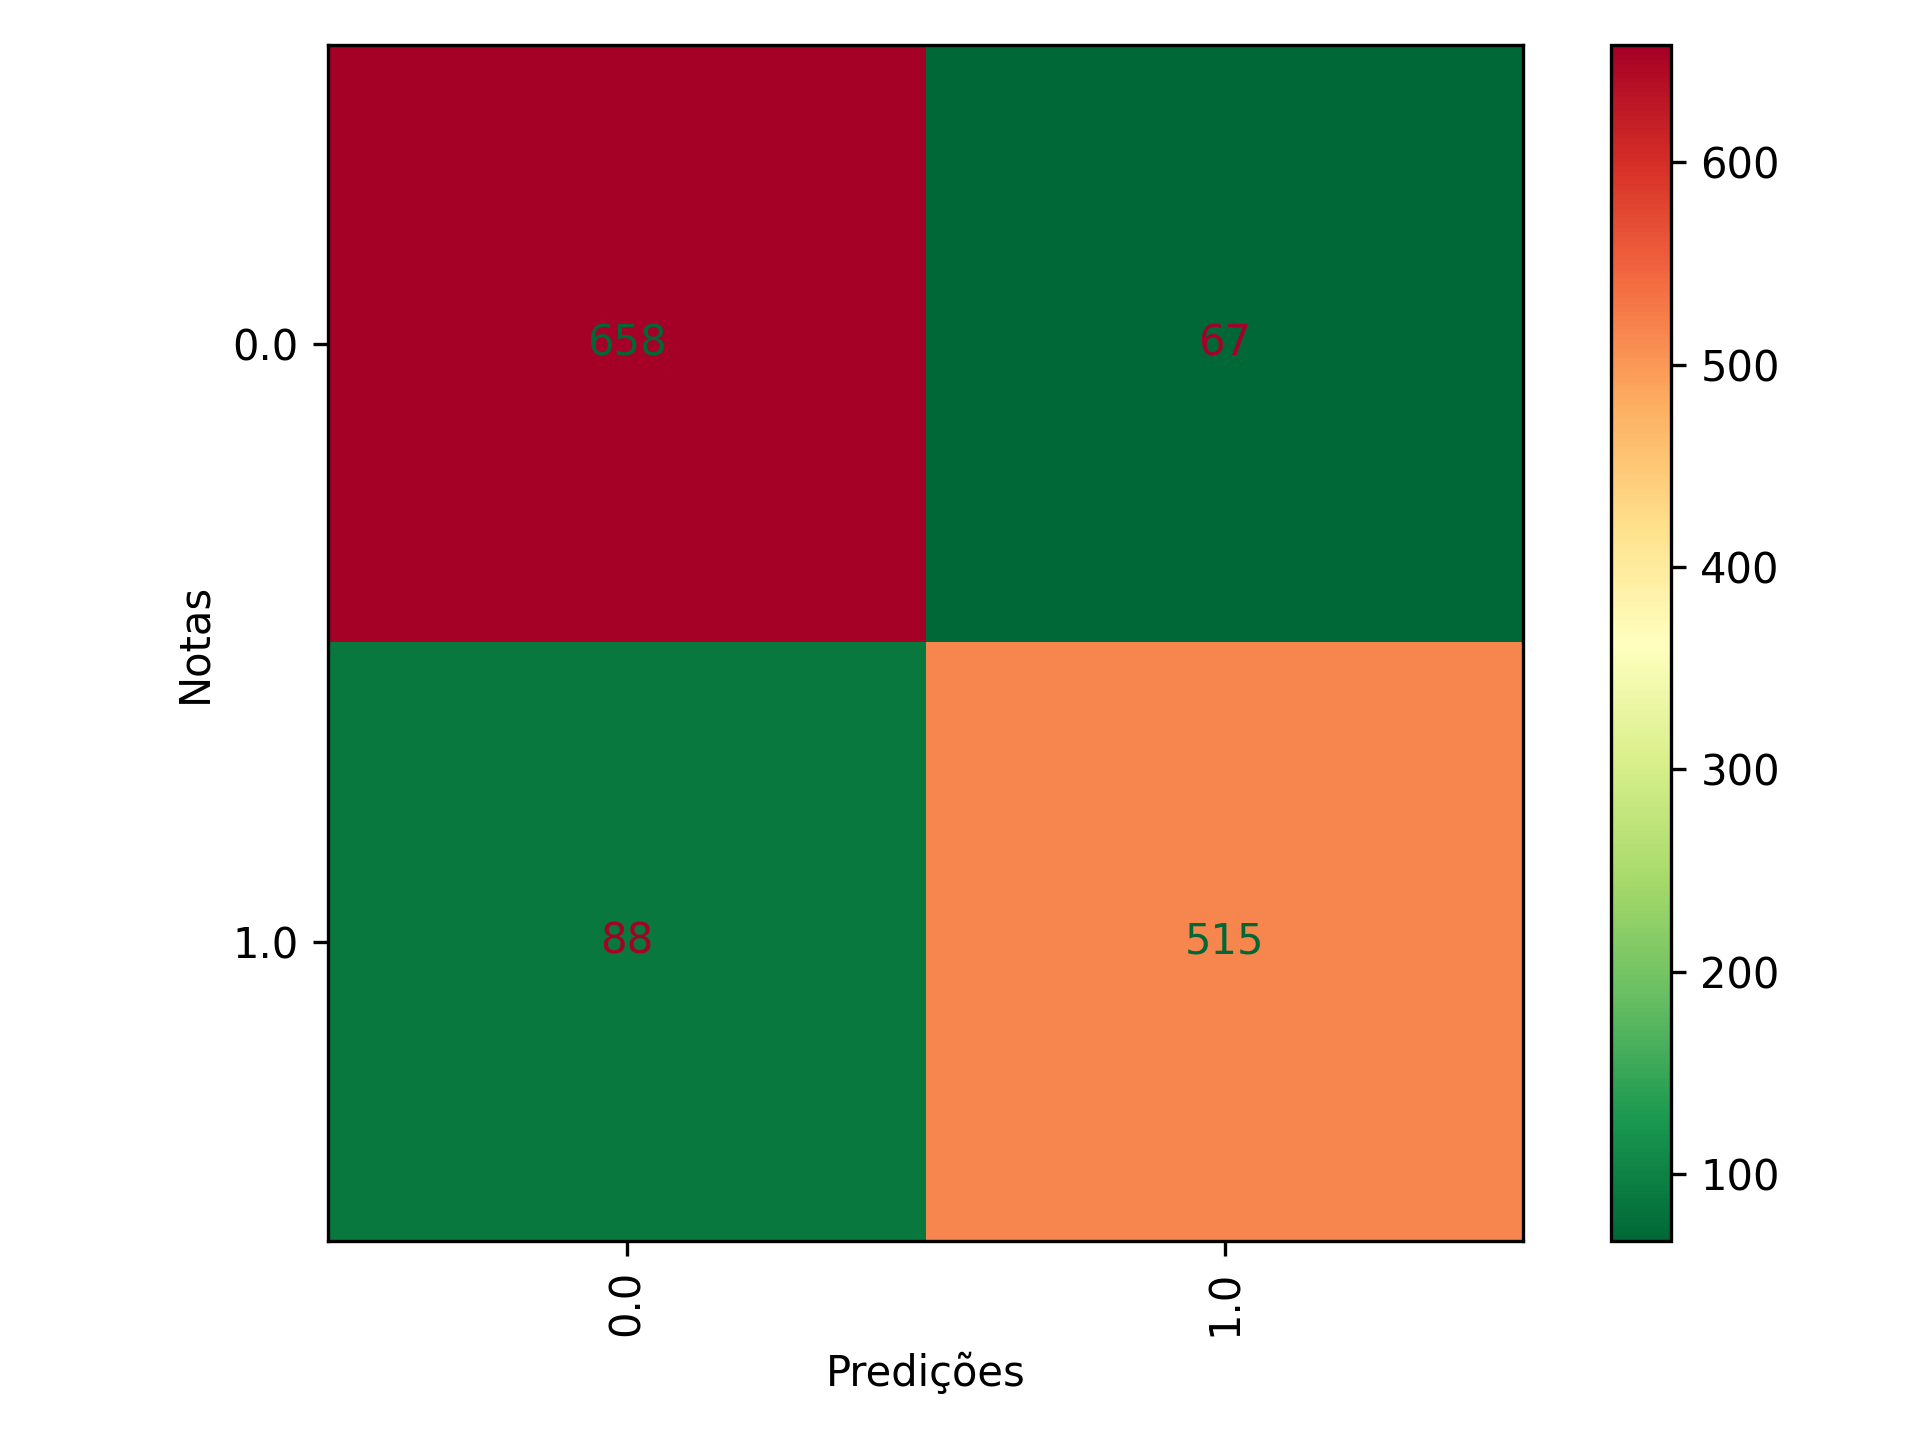
\includegraphics[width=\textwidth]{figuras/exemplo/sandstone-cmRDF.png}
\end{minipage}
\caption{Gráficos exibindo os resultados de classificação do \textit{Random Forest} para a atividade \textit{Sandstone} da \textit{Open University}.}
\label{fig-sandstone-clf}
\end{figure}

Como a Figura \ref{fig-sandstone-clf} retrata, o algoritmo RDF alcançou o índice \textit{avançado} em todas as métricas. Ao professor isso indica que o modelo apresentou alto desempenho, com um método avaliativo muito similar ao atribuído por ele. Alinhado a isto, buscamos caracterizar o método de avaliação de forma a estabelcer para todos os participantes o desempenho obtido. Com isso, esperamos comparar o desempenho inicial com a expectativa de resultados para revisão dos métodos e identificar qualquer falha no sistema. Por conta disso, tais resultados de desempenho são dados quando a atividade encontra-se finalizada e as notas atribuídas são dadas como finais.

\subsection{Identificação de Respostas Candidatas}
\label{subsec-padroes-resposta}

Apesar do acompanhamento da dinâmica do sistema no processo avaliativo, é complexo ao sistema identificar padrões coerentes de resposta. Para isso, utilizamos o quadro de \textit{rubrics} para representar o modelo avaliativo elaborado pelo sistema em conjunto com o professor. O quadro de \textit{rubrics} é um modelo de caracterização do processo avaliativo conforme o modelo de resposta esperado para cada nota. Após o processo avaliativo esse processo torna-se um descritor, determinando na perspectiva dos estudantes quais foram as principais características elencadas para cada nota. 

Para criação do quadro de \textit{rubrics}, ou rúbricas, os exemplos que receberam mesma nota são considerados alinhados com uma expectativa de resposta. Sabendo que o método não utiliza ou compõe respostas candidatas, a ideia é que este processo elenque uma série de respostas para representar cada grau de nota. Para isso, utilizamos o Latent (LDA). O LDA é um método que identifica o grau de correlação do grupo de respostas de mesma avaliação e cada uma das características. A resultante é uma seleção dos 10 principais termos que compõe as respostas selecionadas. Assim, formamos o quadro de \textit{rubrics} organizando as respostas conforme a proximidade de cada uma com as palavras selecionadas. Um exemplo de \textit{rubrics} resultante do processo de identificação da simetria entre termos e notas é dado abaixo. A Tabela \ref{tab-rubrics-exemplo} define o modelo de resposta gerado pelo LDA e as respostas mais similares com o modelo.

\begin{table}
\footnotesize
\begin{minipage}[t]{.45\textwidth}
\begin{tabular}{ p{1.5cm} | p{5cm}}
\hline
\multicolumn{2}{l}{\textbf{Sandstone}} \\ \hline
\multicolumn{2}{c}{\textbf{Nota: 1.0}} \\ \hline 

\multicolumn{2}{l}{\textit{T{\'o}picos: by desert in the wind}} \\ \hline
 \# & Exemplos \\ \hline

53 & \textit{the} sand has been transported \textit{by} \textit{wind} and \textit{the} sandstone probably formed \textit{in} \textit{desert} conditions.\\ \hline
54 & \textit{the} sandstone is a \textit{desert} sand originating \textit{in} a \textit{desert} environment being rounded and sorted \textit{by} \textit{wind} movement.\\ \hline
66 & \textit{the} sandstone originated \textit{in} \textit{the} desert. \textit{the} shape indicates it was transported \textit{by} \textit{wind} and colour indicates oxidisation.\\ \hline
68 & \textit{the} sandstone transported \textit{by} \textit{wind} contains iron which when combined with oxygen gives \textit{the} red colour found \textit{in} \textit{the} desert.\\ \hline
112 & that \textit{the} sandstone originated \textit{in} \textit{the} \textit{desert} and were carried \textit{by} \textit{the} \textit{wind}\\ \hline
377 & \textit{the} rock was formed \textit{in} a \textit{desert} and transported \textit{by} \textit{wind} oxidation of iron has occurred \textit{in} \textit{the} past.\\ \hline
784 & \textit{the} grains from \textit{the} sandstone were transported \textit{by} \textit{wind} \textit{in} oxidising conditions possibly \textit{in} a \textit{desert} situation.\\ \hline
1115 & \textit{the} sand was transported \textit{by} \textit{the} \textit{wind} being deposited \textit{in} \textit{the} air. it comes from \textit{desert} sand \textit{in} oxidising conditions.\\ \hline
1369 & formed \textit{in} a \textit{desert} \textit{in} oxidising conditions and blown \textit{by} \textit{the} \textit{wind} across \textit{the} \textit{desert} causing their well rounded shape.\\ \hline
1826 & it originates \textit{in} \textit{the} \textit{desert} as \textit{the} grains have been transported \textit{by} \textit{wind} and \textit{the} red colour is typical.\\
\\
\\
\hline
\hline
\end{tabular}
\end{minipage} %
\hfill
\begin{minipage}[t]{.45\textwidth}
\begin{tabular}{ p{1.5cm} | p{5cm} }
\hline
\multicolumn{2}{l}{\textbf{Sandstone}} \\ \hline
\multicolumn{2}{c}{\textbf{Nota: 0.0}} \\ \hline 

\multicolumn{2}{l}{\textit{T{\'o}picos: and desert from in the}} \\ \hline
 \# & Exemplos \\ \hline
62 & \textit{the} origin of \textit{the} rock is \textit{from} ancient \textit{desert} deposits \textit{and} has undergone chemical weathering \textit{and} highly oxidising conditions\\ \hline
260 & it says that \textit{the} rock formed \textit{in} \textit{desert} conditions \textit{and} \textit{the} minerals were subjected to heavy chemical weathering \textit{and} erosion.\\ \hline
349 & \textit{the} sand is originally \textit{from} \textit{the} beach \textit{from} \textit{the} wind. \textit{the} colour is \textit{from} iron oxide.\\ \hline
389 & \textit{the} sandstone comes \textit{from} a \textit{desert} \textit{and} contains hematite \textit{from} broken down ferromagnesian minerals \textit{and} oxygen\\ \hline
669 & \textit{the} eviedence suggests that \textit{the} sediment that \textit{the} stone is made \textit{from} originated \textit{in} \textit{the} dessert\\ \hline
670 & \textit{the} sediment that \textit{the} stone is made \textit{from} originated \textit{in} \textit{the} dessert \textit{and} is wind blown \textit{and} contains ironoxide\\ \hline
1037 & \textit{the} sandstone formed \textit{from} \textit{desert} sand dunes \textit{and} was exposed to weathering \textit{and} was not deposited \textit{in} a slow manner.\\ \hline
1236 & \textit{the} sandstone resulted \textit{from} \textit{desert} sediments \textit{the} red colour is \textit{from} insoluble iron entering \textit{the} rock during \textit{the} weathering process.\\ \hline
1331 & originating \textit{from} \textit{the} \textit{desert} as \textit{the} corners are rounded \textit{and} \textit{the} faces are pitted it has an iron oxide coating.\\ \hline
1737 & \textit{the} roundness of \textit{the} grains determines \textit{the} distance \textit{the} sand was displaced \textit{from} \textit{the} source to \textit{the} final deposit.\\ \hline
\hline
\end{tabular}
\end{minipage}
\caption{Tabela de \textit{rubrics} para as duas notas encontradas na atividade exemplo e as respostas mais alinhadas com as palavras selecionadas pelo LDA.}
\label{tab-rubrics-exemplo}
\end{table}

Como podemos observar, na Tabela \ref{tab-rubrics-exemplo}, temos os modelos de resposta para notas 0 e 1. A nota 0 em geral os alunos citam apenas a formação do arenito (\textit{sandstone}) em regiões de deserto. Porém, em um diferencial importante, as respostas detalham a formação através da força do vento. Portanto, a função do \textit{rubrics} é definir os padrões de resposta do sistema e, adicionalmente, criar um relatório que explique o formato avaliativo produzido em conjunto com o professor.

A ideia, portanto, é criar uma visualização do processo avaliativo de acordo com a simetria entre respostas e a avaliação observada pelo sistema. Deste modo, o uso em sala de aula relaciona diretamente cada grau de nota, as principais termos observados nas respostas e os exemplos de resposta coletados dos próprios estudantes. Por fim, como modelo descritivo da avaliação diretamente ao estudante, utilizamos a visualização de correlação entre conteúdo textual e a classificação através do Lime\footnote{Lime - https://github.com/marcotcr/lime}. O Lime é uma ferramenta de visualização que descreve o processo de classificação de acordo com os padrões do conteúdo \cite{ribeiro2016}. Para isso, é apresentado em cada resposta a correlação da resposta e suas principais componentes para cada um dos grupo de nota da avaliação. A Figura \ref{fig-lime-exemplo} apresenta essa estrutura de \textit{feedback} diretamente ao estudante descrevendo sua avaliação.

\begin{figure}[!h]
\centering
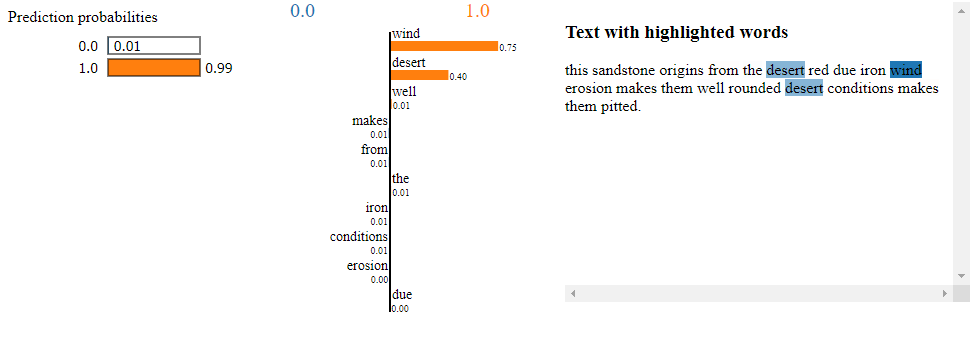
\includegraphics[width=\textwidth]{figuras/exemplo/exemplo-lime}
\caption{Exemplo de uma resposta marcada com palavras identificadas como mais relevantes para a atividade \textit{Sandstone} da \textit{Open University}.}
\label{fig-lime-exemplo}
\end{figure}

Como a resposta da Figura \ref{fig-lime-exemplo} ilustra, podemos identificar o alinhamento das respostas com a atribuição de notas. As palavras em destaque e a correlação de cada uma com a nota caracterizam o processo de classificação automática. Deste modo, o \textit{Lime} foi utilizado para corroborar com o critério avaliativo para que todos acompanhem os resultados encontrados, de forma similar ao \textit{mapa de características} \cite{spalenza2016a}. O processo explicativo para a nota de cada resposta dá ênfase a avaliação produzida em conjunto com o professor. Para além de destacar o possível critério avaliativo em texto, possibilita a discussão dos resultados e a comparação direta entre respostas. Portanto, o material como um todo é importante para o desenvolvimento do ensino-aprendizado para a revisão da questão e para aplicação sala de aula.